\chapter{Experiments}\label{chap:experiments}

This chapter presents experimental results comparing the proposed 1D $k$-means algorithms against the widely used \texttt{scikit-learn} implementation. The evaluation focuses on runtime performance and clustering quality, using both real and synthetic datasets.

\section{Implementation Details}

\sloppy
The proposed algorithms have been implemented as an open-source Python package, \texttt{flash1dkmeans}, available on GitHub\footnote{\url{https://github.com/SyphonArch/flash1dkmeans}} and PyPI\footnote{\url{https://pypi.org/project/flash1dkmeans/}}. The package is built on top of \texttt{NumPy} \cite{numpy} and \texttt{Numba} \cite{numba} for efficient computation. The implementation includes both the $k$-cluster and 2-cluster algorithms, as well as the preprocessing steps for the sorting and prefix sum computations. The preprocessing step is optional and can be disabled if the input data is already in adequate form. More details on the implementation can be found in the Appendix.

\section{Experimental Setup}

The experiments were conducted on two processors: an Intel i9-13900K and an Apple M3. For the clustering quality and runtime comparisons, only the i9-13900K results are presented, as trends were consistent across both processors. Both real and synthetic 1D datasets were used, with varying sizes and numbers of clusters. The real datasets include the \texttt{iris} and \texttt{california housing} datasets from \texttt{scikit-learn}, while synthetic datasets were generated using the \texttt{sklearn.datasets.make\_blobs} and \texttt{numpy.random.random\_sample} functions.

Comparisons were made against \texttt{scikit-learn}'s implementation of $k$-means\footnote{\url{https://scikit-learn.org/stable/modules/generated/sklearn.cluster.KMeans.html}} at default configuration, which utilizes greedy $k$-means++ initialization paired with Lloyd's algorithm. For fair comparison, only a single thread was used. The number of local trials for the greedy $k$-means++ initialization, $l$, defaults to $2 + \log k$ in \texttt{scikit-learn}. This was matched in \texttt{flash1dkmeans}.

\section{Results: Clustering Quality}\label{sec:clustering_quality}

\begin{figure}[H]
    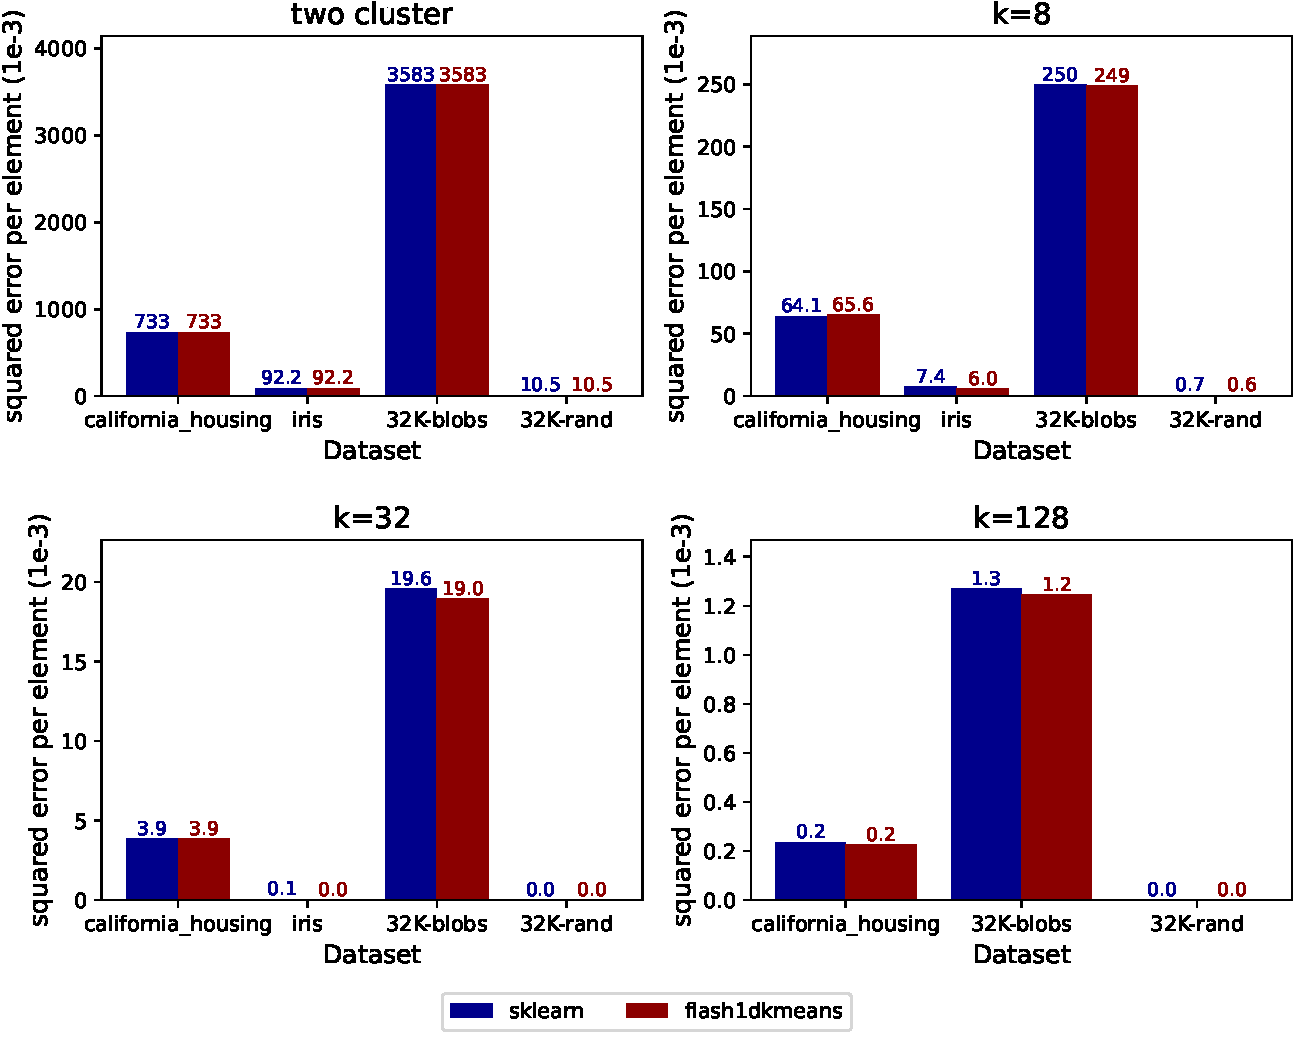
\includegraphics[width=\textwidth]{figures/inertia_comparison.pdf}
    \caption{Squared error comparison of the proposed two-cluster algorithm and $k$-cluster algorithms in \texttt{flash1dkmeans} against \texttt{scikit-learn} on real and synthetic datasets. Lower is better.}
    \label{fig:inertia_comparison}
\end{figure}

The clustering quality comparison between the proposed 2-cluster algorithm and the $k$-cluster algorithms in \texttt{flash1dkmeans} and \texttt{scikit-learn} is shown in Figure~\ref{fig:inertia_comparison}. The \texttt{iris} dataset was excluded for $k=128$ as the number of data points was insufficient. Across the configurations, the clustering quality, measured by squared error, is consistent with the baseline $k$-means algorithm. For both the 2-cluster and $k$-cluster algorithms, this confirms that the proposed method produces clustering results equivalent or close to the $k$-means algorithm in \texttt{scikit-learn}.

\section{Results: Runtime Performance}\label{sec:runtime_performance}

\begin{figure}[H]
    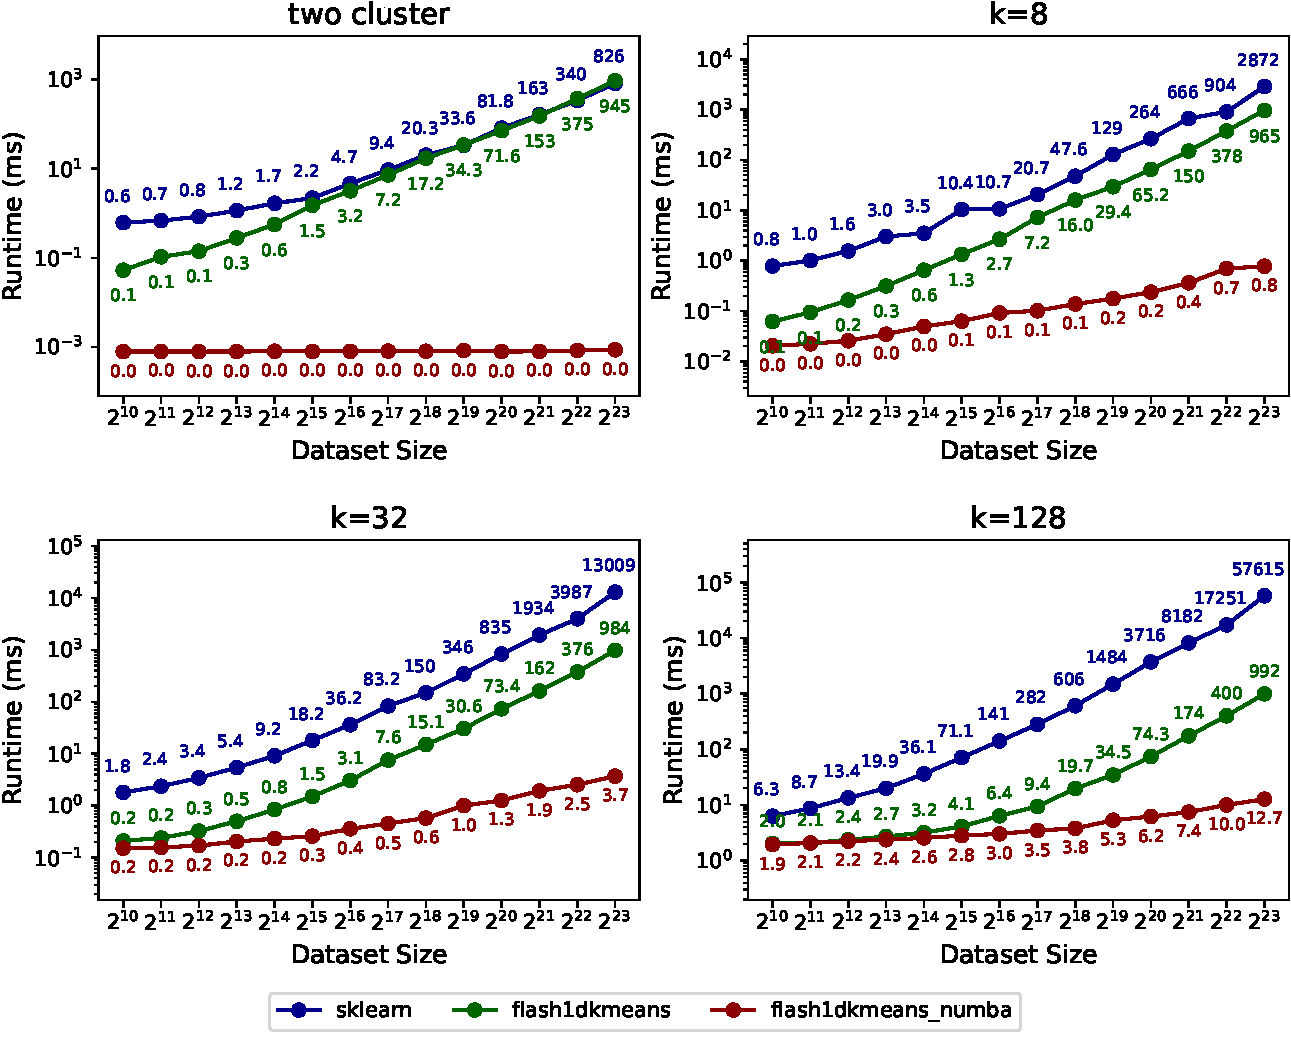
\includegraphics[width=\textwidth]{figures/runtime_comparison.pdf}
    \caption{Runtime comparison of the proposed two-cluster algorithm and $k$-cluster algorithms in \texttt{flash1dkmeans} against \texttt{scikit-learn} on datasets of varying sizes. Lower is better.}
    \label{fig:runtime_comparison}
\end{figure}

Figure~\ref{fig:runtime_comparison} compares the runtime of the proposed 2-cluster and $k$-cluster algorithms in \texttt{flash1dkmeans} to \texttt{scikit-learn}. The runtime of \texttt{flash1dkmeans} includes preprocessing time, while \texttt{flash1dkmeans\_numba} measures only the main algorithm runtime, assuming preprocessed and sorted input data. 

The results confirm that the $k$-cluster algorithm in \texttt{flash1dkmeans} achieves substantial runtime improvements compared to \texttt{scikit-learn}, showcasing the logarithmic dependence on dataset size. For example, for \(k=128\) and dataset size \(2^{23}\), the speedup exceeds 4500x. However, for the 2-cluster algorithm on larger datasets, the \(O(n \log n)\) preprocessing time becomes a bottleneck, limiting the overall speedup. Nevertheless, the main algorithm runtimes confirm the log-time efficiency of the proposed optimizations, and \texttt{flash1dkmeans} with the $O(n \log n)$ preprocessing still outperforms \texttt{scikit-learn} by a large margin in most cases.

\section{Results: LLM Quantization}\label{sec:llm_quantization}

\begin{table}[H]
    \centering
    \resizebox{\linewidth}{!}{%
    \begin{tabular}{|l|c c c|c c c|}
        \cline{2-7}
        \multicolumn{1}{c|}{} & \multicolumn{3}{c|}{\textbf{Seed (k-cluster algorithm)}} & \multicolumn{3}{c|}{\textbf{Upscale (2-cluster algorithm)}} \\
        \hline
        \textbf{Processor} & \textbf{sklearn} & \textbf{flash1dkmeans} & \textbf{speedup} & \textbf{sklearn} & \textbf{flash1dkmeans} & \textbf{speedup} \\
        \hline
        \textbf{i9-13900K} & 433 ms & 56 ms & 7.7x & 10551 ms & 34 ms & 310x \\
        \textbf{Apple M3}  & 572 ms & 114 ms & 5.0x & 7585 ms  & 29 us & 262x \\
        \hline
    \end{tabular}
    }
    \caption{Performance comparison of \texttt{flash1dkmeans} against \texttt{scikit-learn} for both $k$-cluster and 2-cluster algorithms on i9-13900K and Apple M3 processors.}
    \label{tab:anyprec}
\end{table}

Table~\ref{tab:anyprec} compares the performance of \texttt{flash1dkmeans} and \texttt{scikit-learn} in the two-step LLM quantization process proposed in Any-Precision LLM \cite{anyprec}. As an example, we quantize the 214th output channel (size 14,336) of the \texttt{mlp.down\_proj} linear module in the 8th layer of Llama-3-8B \cite{llama3} from 3-bit to 8-bit, as described in the original work. We measure the total time over 100 runs for reliability. 

The first step involves generating a seed model using $k$-means clustering, followed by incrementally subdividing clusters into two via $k$-means in the second step. The preprocessing from the seed generation step is reusable during the upscale phase, enabling the $O(\log n)$-time 2-cluster algorithm to be particularly efficient. Results demonstrate that \texttt{flash1dkmeans} achieves remarkable speedups, surpassing 300x in the upscale step on an i9-13900K processor.

\section{Summary}

Experimental results demonstrate that the proposed algorithms in \texttt{flash1dkmeans} achieve comparable clustering quality to \texttt{scikit-learn} while offering significant runtime improvements. The $k$-cluster algorithm exhibits logarithmic time complexity with speedups exceeding 4500x on large datasets, while the 2-cluster algorithm achieves remarkable efficiency when given preprocessed inputs. These results validate the effectiveness of the proposed optimizations for both general clustering tasks and emerging applications such as LLM quantization.
